\chapter{Resultados dos testes}


\section{Avaliação da Interface}

\indent Os testes foram realizados com 3 biólogos, identificados aqui como Usuário 1, 2 e 3. A Tabela \ref{dados_pessoais} apresenta os dados pessoais de cada um, levando em consideração, principalmente, a experiência que já possuem em redes metabólicas. Isso é necessário, pois quanto mais ele conhecem sobre o conteúdo, mais críticos são a respeito da interface a qual devem interagir em seu trabalho e pesquisas.

\begin{table}[h!]
  \centering
  \caption{Conhecimento dos biólogos selecionados para o teste a respeito dos conceitos utilizados no desenvolvimento da interface do 2Path}
  \label{dados_pessoais}
  \begin{tabular}{lccc}
  & Usuário 1 & Usuário 2 & Usuário 3 \\ \hline
  {\cellcolor[HTML]{DFDFDF}\specialcell{Formação\\acadêmica}} & Possui pós-doutorado & Possui mestrado & Possui metrado \\ \hline
  {\cellcolor[HTML]{DFDFDF}\specialcell{Bancos de\\dados biológicos}} & Conhece bastante & Nunca utilizou  & Conhece \\ \hline
  {\cellcolor[HTML]{DFDFDF}\specialcell{Redes\\metabólicas}} & Conhece bastante & Nunca utilizou & Nunca utilizou  \\ \hline
  {\cellcolor[HTML]{DFDFDF}\specialcell{Ferramentas\\de visualização\\de redes\\metabólicas}} & Conhece bastante & Nunca utilizou  & Nunca utilizou  \\ \hline
  \end{tabular}
\end{table}

\indent Após preencherem o questionário de dados pessoais e conhecimentos do conteúdo a serem expostos, do Anexo \ref{questionario_dados_pessoais}, os biólogos iniciaram as tarefas propostas pelo avaliador, do Anexo \ref{tarefas}. A seguir são listadas todas as principais evidências implícitas e explícitas de falha de comunicação de cada usuário com a interface. Elas estão ordenadas pelo tempo em que aparecem nos vídeos. A etiquetagem foi realizada seguindo os padrões da fase de interpretação de dados do Método de Avaliação de Comunicabilidade, descrito no capítulo 2. As etiquetas são apresentadas na Tabala \ref{tabela_de_etiquetas}.

\indent Análise do \textbf{Usuario 1}:

\begin{itemize}
\item[01:22] Usuário não encontrou as reações que a enzima catalisada, mas logo percebeu que deveria seguir para uma outra página para obter detalhes sobre a busca;
\item[01:26] Usuário se deparou com um grafo em movimento, com 6 nós e cinco arestas, e não entendeu seu significado, a princípio;
\item[01:55] Usuário interagiu com o grafo forçado, pois o mesmo não parava de se mover;
\item[03:50] Usuário diz "Nossa, isso é muito ruim; Não dá pra saber se o substrato da enzima é verde (Composto) ou o rosa (Reação)";
\item[05:10] Usuário tenta entender a legenda do grafo, mas discorda totalmente do proposto;
\item[07:49] Usuário não encontra informação que buscava, até descobrir que deveria seguir para página de detalhes de busca, novamente;
\item[07:53] Usuário expressa desgosto pelo grafo fechado que aparece ao iniciar a página de detalhes da via metabólica;
\item[09:30] Usuário esqueceu de selecionar \textit{Search} e percebeu que havia selecionado em ver detalhes da busca anterior;
\item[10:15] Usuário logo clica no grafo para ele parar de se mover.
\item[ ] \textbf{Fim}. Usuário levou 10 minutos e 44 segundos para finalizar todas as tarefas.
\end{itemize}

\vspace{10mm}
\indent Análise do \textbf{Usuario 2}:

\begin{itemize}
\item[00:41] Usuário percebeu que havia selecionado um botão que não o levava ao seu objetivo;
\item[01:29] Usuário se confunde com função auto-complete do campo de enzimas;
\item[02:01] Usuário demora alguns segundos para perceber que deve seguir para a página de detalhes de busca;
\item[02:20] Usuário demora alguns segundos para entender, a partir da legenda, o significado do grafo que aparece na página de detalhes de busca.
\item[04:55] Usuário não percebe que página retornou sucesso, pois a aparência é de que a mesma não foi atualizada, uma vez que o resultado da busca atual é o mesmo que a busca anterior;
\item[07:55] Usuário tenta impedir grafo de se mover para fora de seu campo de visão;
\item[08:18] Usuário tem dificuldade para entender significado biológico do grafo;
\item[09:30] Usuário esqueceu de selecionar \textit{Search} e percebeu que havia selecionado em ver detalhes da busca anterior;
\item[10:01] Usuário tenta impedir grafo de se mover para fora de seu campo de visão;
\item[10:45] Usuário percebeu que havia errado a tarefa anterior e voltou para refazê-la.
\item[ ] \textbf{Fim}. Usuário levou 11 minutos e 08 segundos para finalizar todas as tarefas.
\end{itemize}

\vspace{10mm}
\indent Análise do \textbf{Usuario 3}:

\begin{itemize}
\item[01:05] Usuário se confunde com função auto-complete do campo de enzimas. Ainda percebe que o problema não é o teclado, mas sim a função que aparece sem necessidade e atrapalha a busca;
\item[01:46] Usuário diz "É só essa a informação?", pois não percebeu, a princípio, que para realizar a tarefa deveria seguir para a página de detalhes da busca;
\item[01:59] Usuário não entende grafo que aparece na tela de detalhes e reclama muito por ele não estar inicialmente parado;
\item[04:20] Usuário reclama da falta de respostas da interface;
\item[06:00] Usuário acha um absurdo o tamanho do grafo que aparece na tela e pede a lista dos detalhes que ele gostaria de saber sobre a busca;
\item[07:20] Usuário reclama da falta de respostas da interface;
\item[07:25] Usuário acha um absurdo o tamanho do grafo que aparece na tela e pede a lista dos detalhes que ele gostaria de saber sobre a busca.
\item[ ] \textbf{Fim}. Usuário levou 7 minutos e 49 segundos para finalizar todas as tarefas.
\end{itemize}

\begin{table}[h!]
  \centering
  \caption{Contabilização das etiquetas para cada usuário. Cada etiqueta é registrada no tempo do vídeo em que ela ocorreu.}
  \label{tabela_de_etiquetas}
  \begin{tabular}{|l|c|c|c|}
  \hline
  {\cellcolor[HTML]{DFDFDF}Etiqueta} & {\cellcolor[HTML]{DFDFDF}Usuário 1} & {\cellcolor[HTML]{DFDFDF}Usuário 2} & {\cellcolor[HTML]{DFDFDF}Usuário 3} \\ \hline
  Desisto. & - & - & - \\ \hline
  Para mim está bom... & - & - & - \\ \hline
  Não, obrigado. & - & - & - \\ \hline
  Vai de outro jeito. & - & - & - \\ \hline
  Cadê? & (01:22), (07:49) & (04:55) & - \\ \hline
  Ué, o que houve? & (09:30) & - & - \\ \hline
  E agora? & - & (02:01) & (01:46) \\ \hline
  Onde estou? & - & - & - \\ \hline
  Epa! & (09:01) & \specialcell{(00:41), (09:30),\\(10:45)} & - \\ \hline
  Assim não dá. & (5:10) & (01:29) & (01:05) \\ \hline
  O que é isto? & (01:26), (03:50) & (02:20), (08:18) & (01:59) \\ \hline
  Socorro! & \specialcell{(01:55), (07:53),\\(10:15)} & (07:55), (10:01) & (06:00), (07:25) \\ \hline
  Por que não funciona? & - & - & (04:20), (07:20) \\ \hline
  \end{tabular}
\end{table}

\indent Após a realização das tarefas, cada biólogo respondeu à um questionário, do Anexo \ref{questionario_interface}, para que fosse avaliado também sua opinião a respeito do sistema.

\indent O usuário 1 relatou que apesar de as tarefas serem relativamente fáceis, a representação das vias metabólicas é confusa, pois a reação é uma ação, portanto seria melhor representada como uma aresta. Quem recebe o substrato e produz outro composto a partir desse é a enzima, portanto o grafo deveria ser configurando mantendo essa informação biológica. Foi reportado, também, que a legenda do grafo estava confusa e poderia conter apenas informações sobre os nós, removendo as informações sobre as arestas, que são óbvias para os biólogos. Por fim, o usuário 1 sugeriu que a via metabólica aparecesse inicialmente estática e com os nós distantes uns dos outros.

\indent O usuário 2 relatou que as tarefas foram fáceis de serem realizadas e didáticas. Segundo ele, praticamente todos os elementos da interface estavam claros, com exceção do grafo, uma vez que entendeu-se que as reações eram arestas.

\indent Por fim, o usuário 3 relatou que as tarefas foram difíceis de serem realizadas, principalmente a segunda, de pesquisar por vias metabólicas entre dois compostos. Na primeira tarefa, o teclado numérico e a função \textit{auto-complete} diminuíram a usabilidade da interface. Já na segunda tarefa, ele seguiu por um caminho diferente do esperado sem perceber, e acidentalmente descobriu um erro no sistema, que retornava dois grafos ao invés de um só. Para justificar seu erro de navegação, ele relatou que não havia percebido a seção de busca no banco de dados completo, à esquerda da pagina de busca. Além disso, assim como o usuário 1, ele sugeriu que a via metabólica aparecesse inicialmente estática e com os nós distantes uns dos outros.

\indent A partir da análise dos três usuários, foram verificados os seguintes pontos fracos do sistema:

\begin{itemize}
\item Busca por enzima / via metabólica
  \begin{itemize}
  \item[1] O botão de voltar um página, do navegador, não fazia o que o usuário esperava. Ele voltava para a pesquisa anterior ao invés de ir para a página central de buscas;
  \item[2] A função \textit{auto-complete} das enzimas não foi uma boa decisão de projeto, pois os usuários ficavam confusos com os números que apareciam;
  \item[3] Resultado de busca não estava sendo inicializado toda vez que página é carregada, portanto apresentava um resultado anterior, o que causava confusão;
  \item[4] Botão \textit{View Interative Data}, para visualizar a via metabólica, esta sempre ativo. Isso fez com que os usuários não notassem que existe informação extra sobre enzima ou via quando a pesquisa retorna sucesso;
  \item[5] Botões \textit{Search} e \textit{View Interative Data} estavam muito próximos um do outro. Usuários às vezes não selecionavam o botão \textit{Search} antes de clicar em \textit{View Interative Data}, pois a segunda coluna da página estava mal localizada, para um formulário;
  \item[6] A página de busca central dá mais foco em busca por elementos no organismo, e isso faz com que a seção menor à esquerda passe despercebida.
  \end{itemize}

\item Visualização do grafo
  \begin{itemize}
  \item[1] A reação não deveria ser representada por um nó, pois para os biólogos, ela é uma ação, e não um elemento. Assim, faz mais sentido biológico uma aresta saindo do substrato para a enzima, e saíndo da enzima para o produto. A aresta entre enzima e reação não é necessária. Houve muita confusão, pois pensaram que reação era representada por aresta invés de nó;
  \item[2] Não é necessário apresentar os nós do organismo e sequências que o organismo possui. Ao apresentar a enzima na busca de informações no organismo, já é implícito que aquela enzima é produzida pelo organismo;
  \item[3] Quanto maior o grafo, mais complexo é entendê-los;
  \item[4] Grafos muito grades podem ficar cortados e alguns elementos podem sair do campo de visão do usuário.
  \item[5] É mais desejável um grafo que apareça primeiramente de maneira estática. Um grafo que aparece se movendo levemente é irritante. Caso o usuário queira mover e clicar nos elementos, ele o faz com mais facilidade com um grafo estático;
  \item[6] É mais agradável um grafo que apareça aberto;
  \item[7] As labels poderiam apresentar só as bolinhas e explicação a respeito do que elas representam. A informação sobre as arestas já é informação extra desnecessária;
  \end{itemize}
\end{itemize}


\indent Além dessas dificuldade relatadas, foi encontrado um \textit{erro} de implementação em um dos testes. Uma das tarefas era encontrar uma via metabólica entre dois compostos no grafo completo do 2Path, porém um dos usuários utilizou a busca por via em um organismo. A busca deveria retornar que não há via, porém ela retornou que existia, e apresentou um grafo disjunto\footnote{Dois grafos que não se conectam.}. Um grafo era do organismo com todas as enzimas que ele produzia e o outro grafo representava a via entre os compostos pesquisados.

\indent A seguir está uma lista de mudanças no projeto de interface, feita após os testes do Método de Avaliação de Comunicabilidade. Cada item representa a solução dos problemas relatados na lista anterior.

\begin{itemize}
\item Busca por enzima / via metabólica
  \begin{itemize}
  \item[1] Foi adicionado um botão de voltar nas páginas específicas de busca por enzima e vias metabólicas, assim o usuário pode clicar nele e voltar diretamente para a página de buscas gerais;
  \item[2] A função \textit{auto-complete} do campo de busca por enzima foi removida;
  \item[3] As mensagens de sucesso e erro são apresentadas no canto superior direito da tela e são atualizadas sempre que uma nova busca é feita. Ela aparece por 5 segundos e depois desaparece.
  \item[4, 5] O grafo que apresenta os detalhes sobre a enzima ou via metabólica buscada aparece na mesma página que o formulário de pesquisa. Se a busca retorna verdadeira, o grafo aparece, se retorna falsa, não aparece. Assim, o usuário não precisa seguir mais um passo na interface para visualizar os dados biológicos que procura;
  \item[6] As colunar de busca no banco completo e no organismo foram configuradas no mesmo tamanho e ícones que simbolizam elementos públicos e privados foram posicionados ao lado dos títulos de cada busca.
  \end{itemize}
  
\item Visualização do grafo
  \begin{itemize} 
  \item[1] NÃO DÁ: Uma enzima pode catalisar mais de uma reação. Assim, não teria como representar o nó da enzima recebendo todos os possíveis substratos e produzindo todas os possíveis produtos. Seria mais fácil pedir pro waldeyr adicionar uma propriedade no nó da reação falando qual enzima catalisa a reação.
  \item[2, 3, 4] Para diminuir o tamanho do grafo, foram omitidos os nós referentes ao organismo e às sequências do genoma que ele possui.
  \item[5] O grafo aparece estático, porém o usuário pode clicar nos nós e movê-los como desejar;
  \item[6] O nós do grafo não se sobrepõem, portanto ele tem a aparência de que está aberto;
  \item[7] A legenda apresenta apenas informações sobre as cores de três nós: Compostos, Reações e Enzimas;
  \end{itemize}
\end{itemize}
 
 
 
% Telas, printscreen

\section{Nova Interface do Sistema}

\begin{figure}[!h]
    \centering
    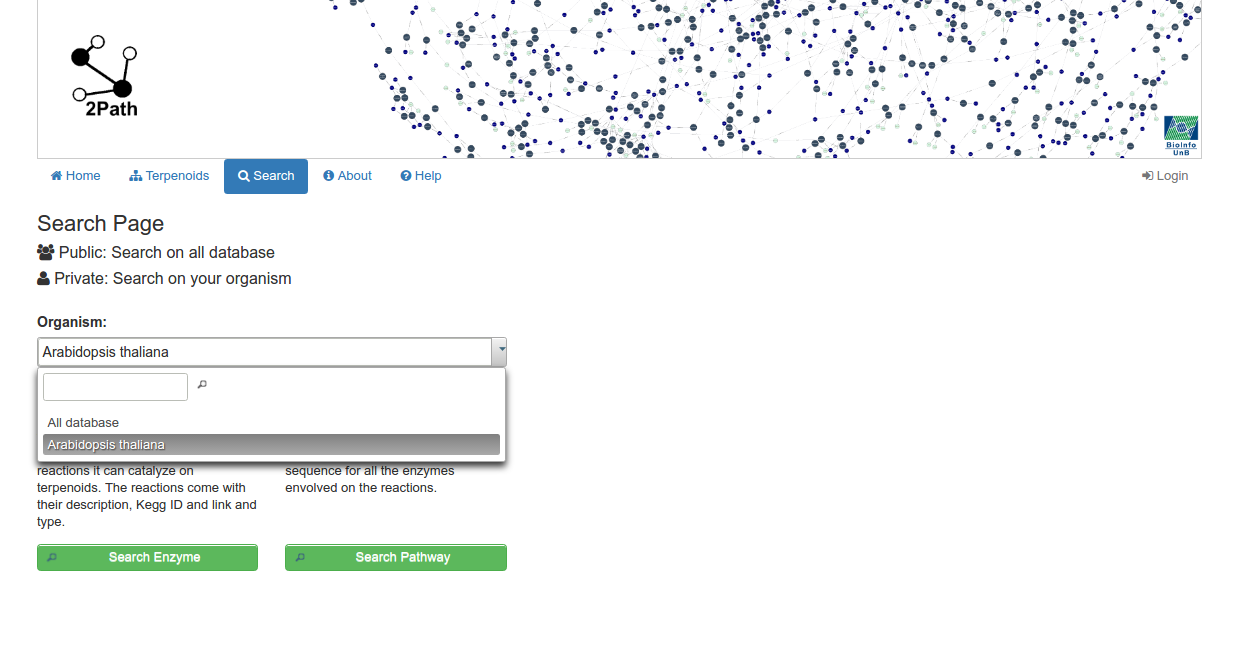
\includegraphics[width=1\textwidth]{new_search_page.png}
    \caption{}
    \label{fig:new_search_page}
\end{figure}

\begin{figure}[!h]
    \centering
    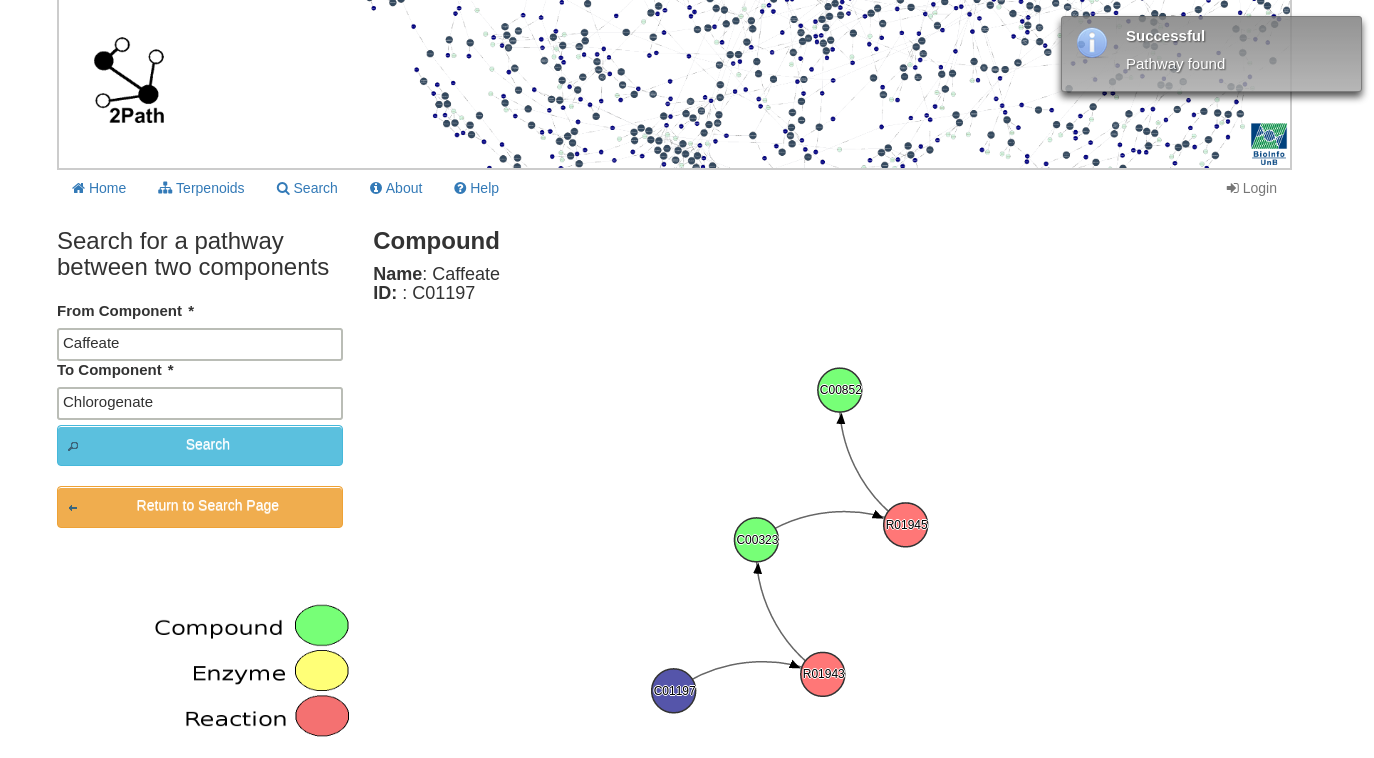
\includegraphics[width=1\textwidth]{new_message_success.png}
    \caption{}
    \label{fig:new_message_success}
\end{figure}

\begin{figure}[!h]
    \centering
    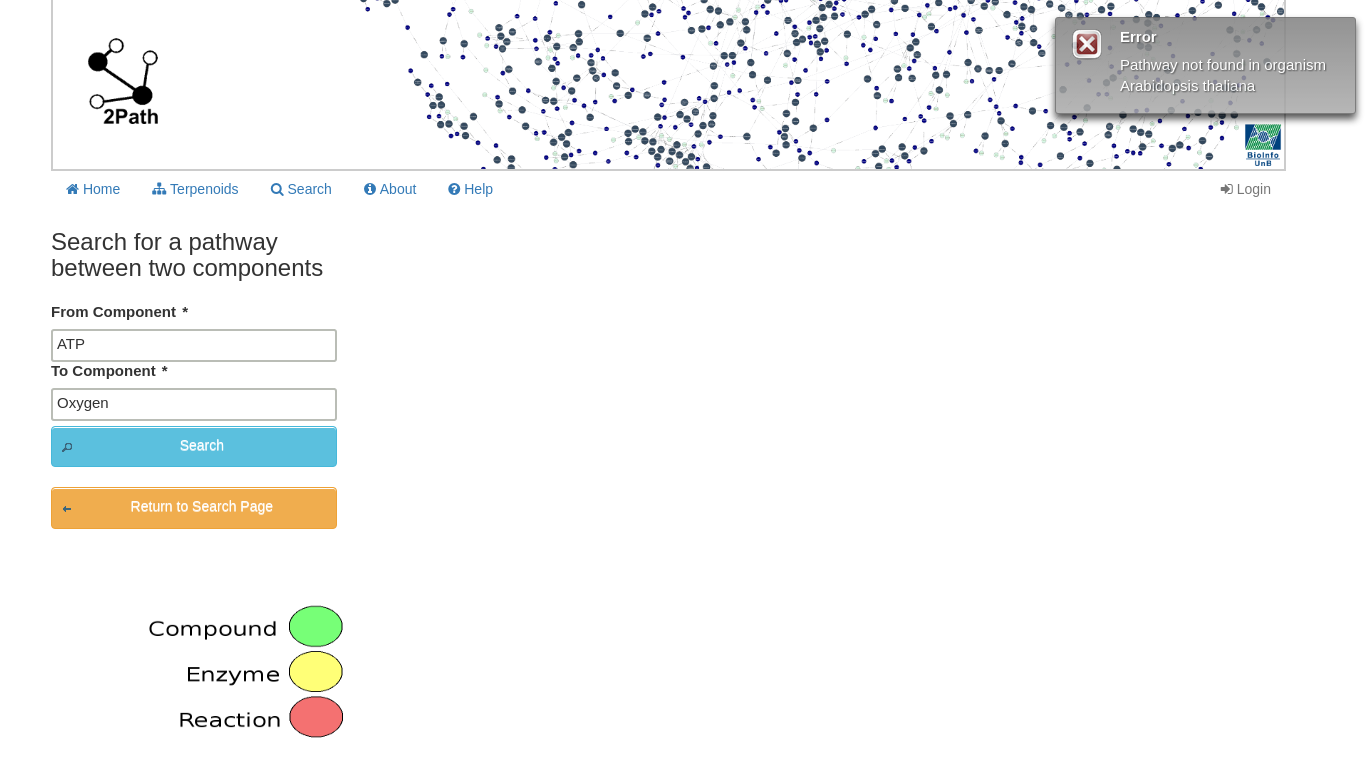
\includegraphics[width=1\textwidth]{new_message_error.png}
    \caption{}
    \label{fig:new_message_error}
\end{figure}

\begin{figure}[!h]
    \centering
    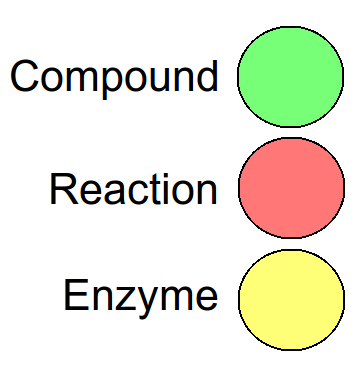
\includegraphics[width=0.2\textwidth]{new_legenda.png}
    \caption{}
    \label{fig:new_legenda}
\end{figure}

\begin{figure}[!h]
    \centering
    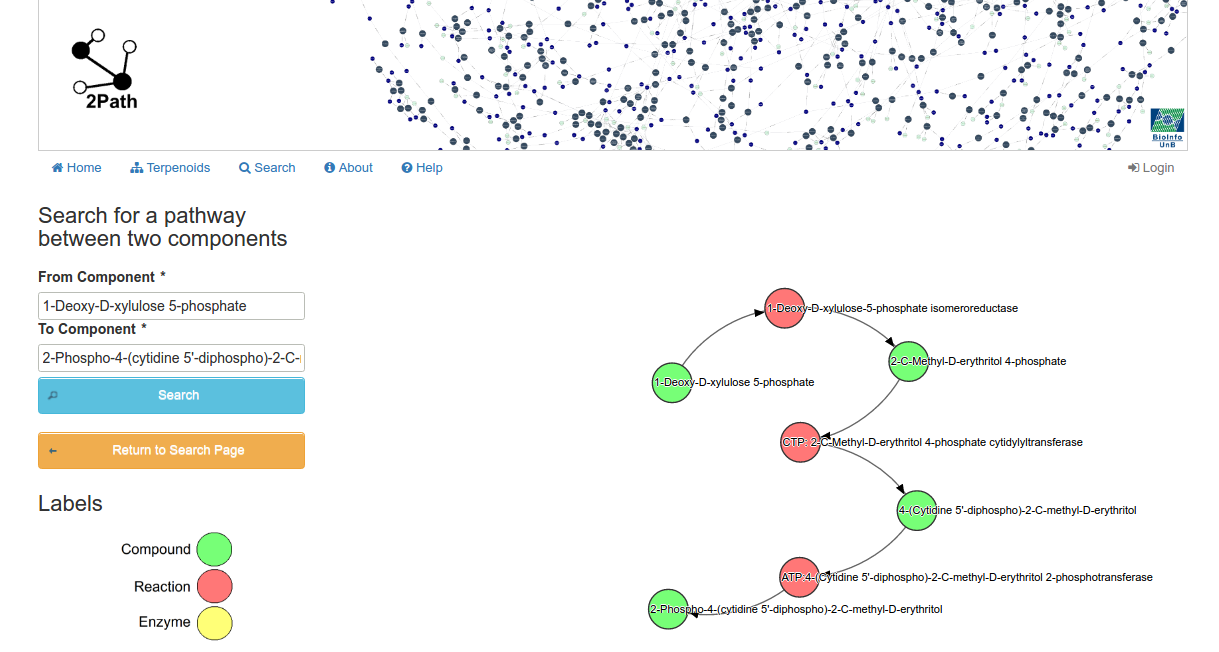
\includegraphics[width=1\textwidth]{new_pathway.png}
    \caption{}
    \label{fig:new_pathway}
\end{figure}

\begin{figure}[!h]
    \centering
    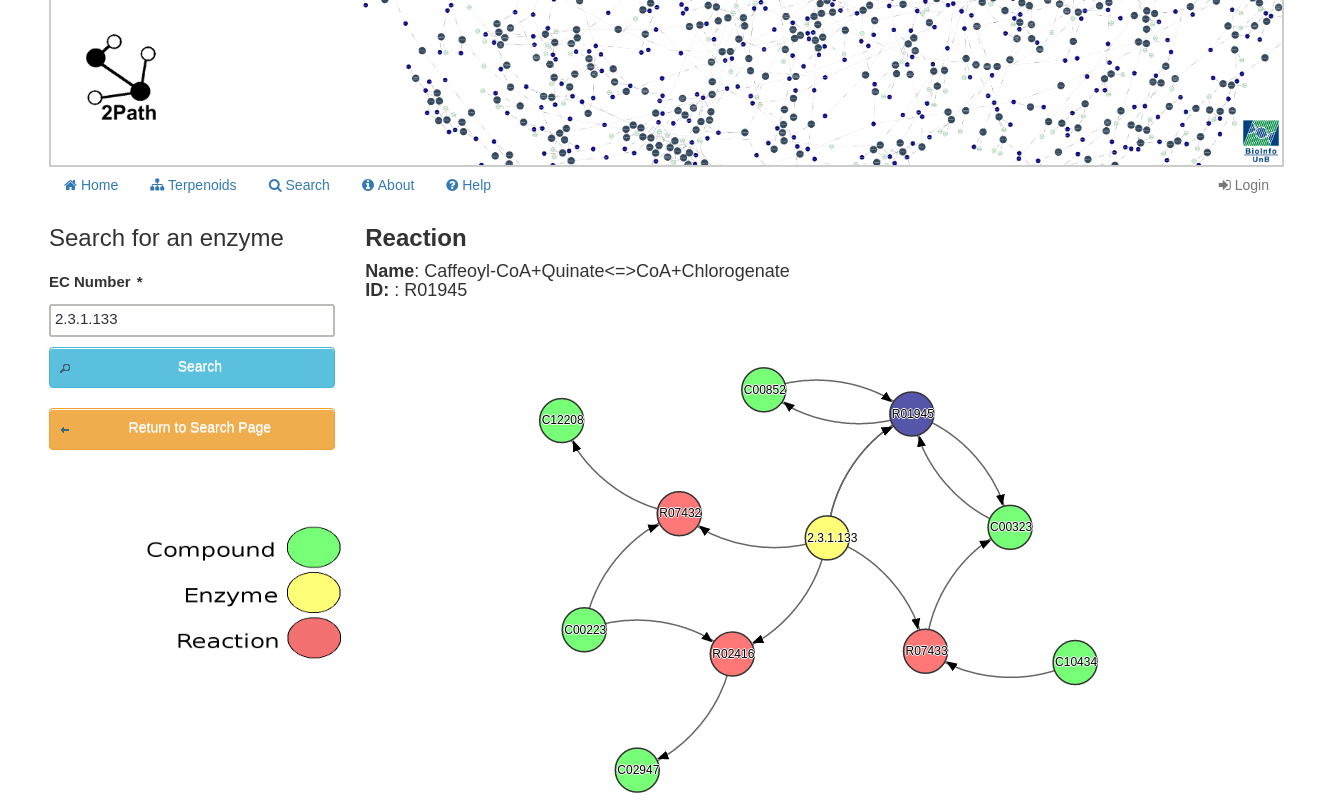
\includegraphics[width=1\textwidth]{new_enzyme_4_catalyses.png}
    \caption{PROBLEMA: ENZIMA PODE CATALIZAR MAIS DE UMA REACAO}
    \label{fig:new_enzyme_4_catalyses}
\end{figure}


